\documentclass{beamer}

\usepackage{graphics}
\usepackage{graphicx}
\usepackage{float}
\usepackage{caption}
\usepackage{subcaption}
\usepackage{color}

\usetheme{Szeged}
\usecolortheme{beaver}

\beamertemplatenavigationsymbolsempty
\frenchspacing
\setbeamertemplate{itemize item}{\color{black}\textbullet}
\usefonttheme{serif}

\captionsetup[figure]{labelformat=empty}
\captionsetup[subfigure]{labelformat=empty}

\newcommand\frametitlesc[1]{\frametitle{\sc #1}}

\newcommand\ee{\boldsymbol{e}}
\newcommand\prn[1]{\left( #1 \right)}
\newcommand\set[1]{\left\{ #1 \right\}}


\title[short title]{\sc Title}
\author{Cody Buntain, Christopher Natoli, Miroslav \v{Z}ivkovi\'{c}}
\date{24 July 2014}
\institute[OSDC PIRE 2014 at UvA]{OSDC PIRE 2014, hosted at University of Amsterdam}

\begin{document}

\frame{\titlepage}

\section{Introduction}

\section{Algorithms}

\subsection{Likelihood ratio}

\frame{
  \frametitlesc{Title}
  \begin{itemize}%\itemsep=0.5cm
  \item item
  \end{itemize}
}

\subsection{Cusum}

\frame{
  \frametitlesc{Building the test statistic}
  $$
  \mathrm{test\;statistic}=
  \onslide<5->{\frac{h}{\sqrt{2kn}}\bigg(}
  \frac{
    \onslide<1->{\sum_{t=1}^h\ee_t}
    \onslide<2->{^\top}
    \onslide<3->{(\hat\Sigma)^{-1}}
    \onslide<2->{\ee_t}
  }{\onslide<3->h}
  \onslide<4->{-\frac{\sum_{t=1}^n\ee_t^\top(\hat\Sigma)^{-1}\ee_t}{n}}
  \onslide<5->{\bigg)}
  $$
  \onslide<3>{$$\hat\Sigma:=\frac{1}{n-1}\sum_{t=1}^n\ee_t\ee_t^\top$$}
}

\frame{
  \frametitlesc{Finding a single changepoint}
  \begin{figure}
    \centering
    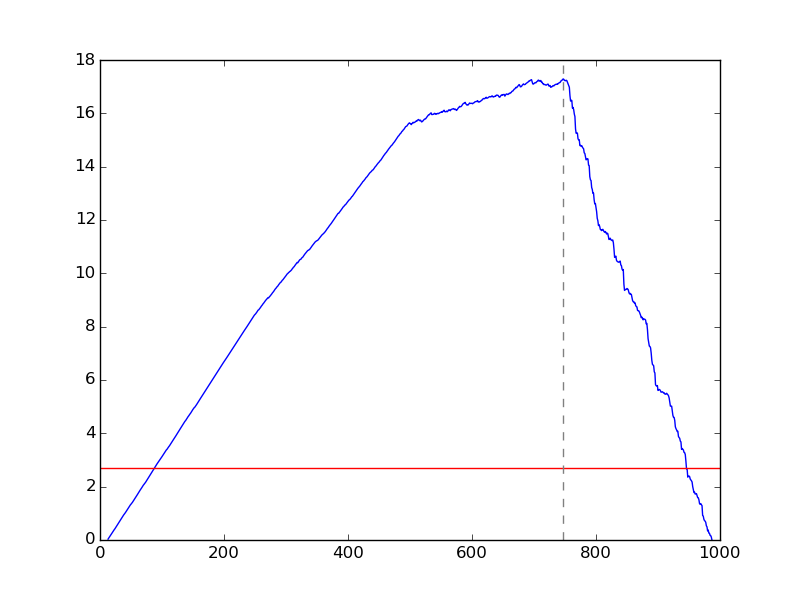
\includegraphics[width=.7\textwidth]{cusum_plot1.png}
    \caption{Cusum statistic for a time series with three changepoints.}
  \end{figure}
}

\frame{
  \frametitlesc{Finding a single changepoint}
  \footnotesize
  \begin{align*}
  \max(\mathrm{test\;statistic})
  &=\max\prn{\frac{h}{\sqrt{2kn}}\bigg(\frac{\sum_{t=1}^h\ee_t^\top(\hat\Sigma)^{-1}\ee_t}{h}-\frac{\sum_{t=1}^n\ee_t^\top(\hat\Sigma)^{-1}\ee_t}{n}\bigg)}\\
  &\xrightarrow{D}\sup\set{\text{Brownian bridge}},
  \end{align*}
  which is a known distribution!
}

\frame{
  \frametitlesc{Finding more changepoints}
  \begin{figure}
    \centering
    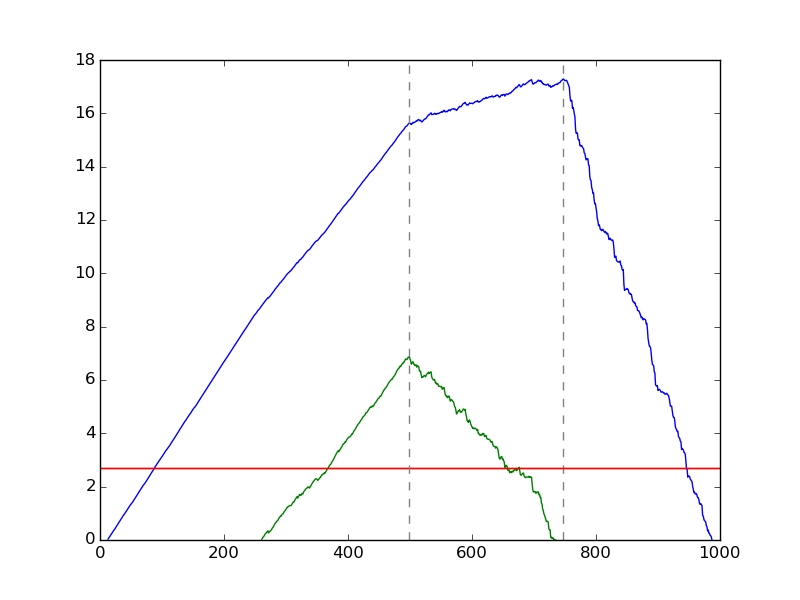
\includegraphics[width=.7\textwidth]{cusum_plot2.png}
    \caption{Cusum statistic for a time series with three changepoints.}
  \end{figure}
}

\subsection{Kernel changepoint detection}

\frame{
  \frametitlesc{Title}
  \begin{itemize}%\itemsep=0.5cm
  \item item
  \end{itemize}
}

\subsection{Density ratio estimation}

\frame{
  \frametitlesc{Title}
  \begin{itemize}%\itemsep=0.5cm
  \item item
  \end{itemize}
}

\section{Other stuff}

\end{document}
